%%This is a very basic article template.
%%There is just one section and two subsections.
\documentclass{article}

\usepackage{graphicx}
\usepackage[utf8]{inputenc}
\usepackage{ngerman}
\usepackage{algorithmic}

\begin{document}


\newcommand{\HRule}{\rule{\linewidth}{0.5mm}}



\begin{titlepage}

\begin{center}




\textsc{\LARGE QuDiMo - Internal Document}\\[1.5cm]

\textsc{\large University of Siegen}\\
\textsc{\large Software Engineering Group}\\[0.5cm]


\HRule \\[0.4cm]
{ \huge \bfseries SiDiff Matching Configuration} \\[0.4cm]

\HRule \\[1.5cm]

\emph{Author:} MR, PP\\


\vfill
\begin{center}
  \begin{tabular}{| c || c | c | c | }
    \hline
    Date & Version & Initials & Comments\\ \hline
    2012.01.16 & 0.1 & MR & Initial Version \\ \hline
    2014.10.09 & 0.1 & MR & Strukturierung, Korrekturen, Encoding, Ergänzungen
    \\
    \hline - & - & - & -\\
    \hline
  \end{tabular}
\end{center}
% Bottom of the page
{\large \today}

\end{center}

\end{titlepage}

\section{Einleitung}

In SiDiff gibt es drei Konfigurationen.
Die wesentlichsten sind jedoch die CompareConfiguration (a.k.a.
Vergleichskonfiguration) und die Matchingkonfiguration.
\\\\
Die Vergleichskonfiguration gibt im wesentlichen an, mit welchen Hilfsmitteln
einzelne Elemente, Attribute, Referenzen verglichen werden (also z.B. ob ein
String, Integer, \ldots., EObject-Vergleich genutzt werden soll).
Auf der Vergleichskonfiguration werden Schwellwerte (``thresholds'') für jeden
Modellelementtyp definiert. Damit zwei Elemente aus unterschiedlichen
Modellinstanzen als \textit{Kandidaten} für eine potentielle Ähnlichkeit
markiert werden können, muss beim Vergleich mit den angegebenen Hilfsmitteln der Vergleichs-threshold
erreicht werden.
\\\\
Die Matchingkonfiguration definiert im Wesentlichen, ab wann zwei Elemente,
welche zuvor als ähnliche Kandidaten markiert wurden, tatsächlich auch als
Korrespondenzen zueinander erkannt werden. Dazu werden auf der
Matchingkonfiguration auch sogenannte ``thresholds'' erreicht. Diese sind in
der Regel höher angesetzt als die thresholds auf der Vergleichskonfiguration.
\\\\
Dieses Dokument geht auf die Details der Matchingkonfiguration ein.

\section{Struktur}
Eine Matchingkonfiguration entspricht der folgenden Stuktur.
Die in Großbuchstaben markierten Platzhalter genauer weiter unten genauer
erklärt.
\begin{verbatim}
<Matching>

	<Settings defaultSequencedMatcher="A_MATCHER"
		   defaultTopDownMatcher="A_TOP_DOWN_MATCHER"
		   documentType="METAMODEL_URI"
		   firstPassSequencedMatcher="A_MATCHER"
		   matcherPrefix="PACKAGE_NAME" />

	<Configurations>
		<MatchingConfiguration	 className="MODEL_ELEMENT"
					 allowGlobalMove="true_OR_false"
					 alwaysComputeSimilarity="true_OR_false" 			
					 independentMatching="true_OR_false" 
					 threshold="DECIMAL_VALUE" 
					 topDownMatcher="A_TOP_DOWN_MATCHER"
		</MatchingConfiguration>
		...
	</Configurations>
	<Sequence>		
		<Class name="MODEL_ELEMENT" />
		...
		<Sequence initial="2">
			<Class name="MODEL_ELEMENT" />
			...
		</Sequence>
	</Sequence>
</Matching>
\end{verbatim}

\paragraph{A\_MATCHER}

Ein Matcher aus dem Plugin org.sidiff.core.matching.iterative,
genauer: aus dem Package org.sidiff.core.matching.matcher. Es sind folgende speziellere
Matcher möglich:
\begin{enumerate}
  \item \textbf{DefaultMatcher}
  Liefert den (einen) "ahnlichsten Kandidaten eines
  Objekts aus einer Kandidatenliste, welcher auch den Threshold überschreiteten
  muss.
  \item \textbf{GreedyParentForcedMatcher}
  Liefert den (einen) ähnlichsten
  Kandidaten eines Objekts aus einer Kandidatenliste. Wenn der Elternknoten gematcht wurde,
  dann wird das matchen der Kinder ``erzwungen''. Dabei werden alle Kinder der
  gematchten Elternknoten einander zugeordnet. Es wird nicht geprüft, ob der
  Ähnlichkeitswert gleich dem Threshold ist oder ihn überschreitet.
  \item \textbf{NoMatcher}
  Ein bottom-up-matcher, der nichts matcht.
  \item \textbf{UniqueSimilarityMatcher}
  Liefert den einzigen existierenden Kandidaten,
  welcher auch mindestens den Threshold erreichen muss. Wenn es nur einen Kandidaten
  gibt, der eine Ähnlichkeit über dem Threshold aufweist.
\end{enumerate}


\paragraph{METAMODEL\_URI}
Die Meta-Modell Namespace URI.
Kann zum Beispiel sein: http://www.eclipse.org/uml2/3.0.0/UML

\paragraph{PACKAGE\_NAME} 
Her steht lediglich der Namespace, welcher den Matcher enthält.
Also in der Regel ``org.sidiff.core.matching.matcher''.

\paragraph{A\_TOP\_DOWN\_MATCHER}
Beim Matchingvorgang werden Modelellemente in der Modellinstanz ausgehend von
der Wurzel bis zu den Blättern betrachtet. Der Matcher liegt in dem
Plugin org.sidiff.core.matching.iterative,
genauer: aus dem Package org.sidiff.core.matching.matcher. Möglich speziellere
Top-down Matcher:

\begin{enumerate}
  \item \textbf{Propagation}
  Liefert das Element mit dem höchsten Ähnlichkeitswert
  zum ausgewählten Objekt. Der Threshold muss mindestens erreicht werden. Außerdem
  werden die Ähnlichkeitswerte für ein Objekt nicht (?) aktualisiert.
  \item \textbf{NoPropagation}
  Top-Down-Matcher, der nichts matcht, aber dafür genutzt
  wird, eine Propagation nach unten zu unterbinden.
  \item \textbf{UniquePropagation}
  Matcht Kindelemente, solange für diese jeweils nur
  eine Ähnlichkeit zu einem anderen Kind existiert. Außerdem werden die
  Ähnlichkeitswerte für ein Objekt aktualisiert.
  \item \textbf{GreedyPropagation}
  Liefert das Element mit dem höchsten
  Ähnlichkeitswert zum ausgew"ahlten Objekt. Der Threshold spielt keine Rolle.
  Außerdem werden die Ähnlichkeitswerte für ein Objekt aktualisiert.
  \item \textbf{GreedyForcedPropagation}
  Liefert das n"achstbeste Element mit
  irgendeinem Ähnlichkeitswert zum ausgew"ahlten Objekt. Außerdem werden die
  Ähnlichkeitswerte für ein Objekt aktualisiert.
\end{enumerate}



\paragraph{``MODEL\_ELEMENT''}:
MatchingConfiguration bezieht sich auf angegebenen Modelelementtyp.

\paragraph{allowGlobalMove=``true\_OR\_false''}:
Option, um globale Verschiebung des Elements beim Matching (nicht)
berücksichtigen. Elemente vom gleichen Typ werden nicht gematcht wenn
sie sofern sie in anderen Kontexten liegen.

\paragraph{alwaysComputeSimilarity=``true\_OR\_false''}: Option, um den
Ähnlichkeitswert nach jeder Ergänzung an der Kandidatenliste (nicht) neu
zuberechnen. Mit anderen Worten: (nicht) jedesmal die Ähnlichkeitsneuberechnung
durchzuführen, wenn andere Modelelemente gematcht wurden.

\paragraph{independentMatching=``true\_OR\_false''}: ?

\paragraph{threshold=``DECIMAL\_VALUE''}: Schwellwert, der erreicht werden muss,
damit eine endgültige Korrespondenz vorliegen kann. Je höher der Dezimalwert,
desto niedriger die Wahrscheinlichkeit, dass Korrespondenzen für diesen
Modelelementtyp gefunden werden.

\paragraph{topDownMatcher=``A\_TOP\_DOWN\_MATCHER''}: Angabe, welcher TopDownMatcher
genutzt werden soll (Siehe Bild unten)

\paragraph{Erläuterung des Sequence-Tags}
Eine Sequenz gibt die Reihenfolge an, in der die Modelelemente zur
Ähnlichkeitsberechnung abgearbeitet werden. Die Seqzenzen bieten damit eine
Erweiterung zu dem Top-Down/Bottom-Up Matchern, insbesondere wenn
Geschwister-Knoten vorang gewährt werden soll oder wenn im
Top-Down/Bottom-Up Matchingverfahren Ausnahmen in der Reihenfolge für
bestimmte Modellelementtypen getätigt werden sollen. Wenn Propagation genutzt
wird, beeinflusst der aktuell errechnete Ähnlichkeitswert hinsichtlich zweier
Elemente in der Instanz alle deren Kind- und Eltern-Elemente: Ähnlichkeitswerte der Kinder- bzw.
Elternelemente werden mit dem aktuell errechneten Ähnlichkeitswert jeweils
summiert. Letzeres kann also u.U. ermöglichen, dass Thresholdwerte der
Kinder-/Elternelemente nun erreicht werden können, falls die
Ähnlihchkeitsberechnung dieser alleine nicht zu einer Korrespondenz geführt hat.

\paragraph{initial}
Initial gibt die Anzahl der Durchläufe der Sequence an, bevor das eigentliche
Matching geschehen soll. Es werden also initial nur Kandidaten für Matchings
erstellt, bevor diese Kandidaten zu Korrespondenzen werden (Dies wird
entschieden über den Threshold-Wert in der MatchingConfiguration).
Die ``initial"-Angabe macht nur Sinn, wenn Propagation genutzt wird.

\section{Hierachie der Matcher}
\begin{center}
\begin{figure*}[htb!]
  \centering
       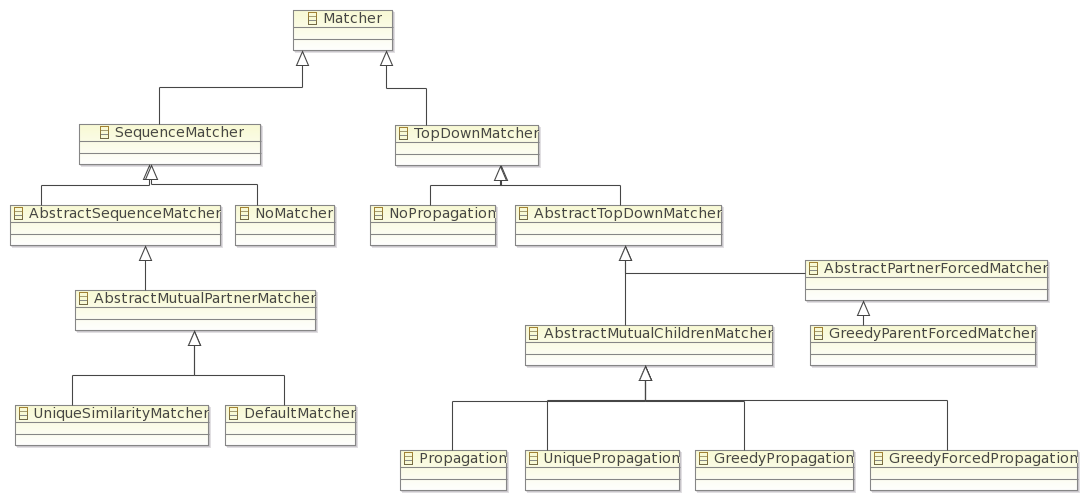
\includegraphics[width=\textwidth]{pics/matcher.png}
  \caption{Matcher Hierachie - Overview}
  \label{fig:overview}
\end{figure*}
\end{center}
\end{document}
